\section{Kontextabgrenzung}

\subsection{Fachlicher Kontext}

Die E-Commerce-Plattform wird von registrierten und nicht registrierten Benutzern verwendet.
Nicht registrierte Benutzer können Produkte suchen und anzeigen sowie ein Benutzerkonto erstellen.
Registrierte Benutzer können zusätzlich Produkte einstellen und kaufen.

Nach einem erfolgreichen Kauf wird eine Bestellbestätigung über einen externen E-Mail-Dienst versendet.


\subsection{Technischer Kontext}

Das System tritt nach außen als eine zusammenhängende Anwendung auf und wird über einen Webbrowser genutzt.
Das Frontend kommuniziert über HTTP/REST mit dem API Gateway, das den zentralen Einstiegspunkt bildet.

Die interne Kommunikation zwischen den Services erfolgt über REST und MQTT.
Die externen Schnittstellen sind in
Tabelle~\ref{tab:externe_schnittstellen} dargestellt.

\subsection{Externe Schnittstellen}

\begin{table}[ht]
    \centering
    {
        \renewcommand{\arraystretch}{1.5}
        \rowcolors{2}{tableRowColor}{white}


        \begin{tabularx}{\linewidth}{
                >{\bfseries\raggedright\arraybackslash}p{0.20\linewidth}
                >{\raggedright\arraybackslash}p{0.18\linewidth}
                >{\raggedright\arraybackslash}X
        }
        \toprule
        Gegenstelle & Richtung & Inhalt und Protokoll \\
        \midrule

        Webbrowser &
        Bidirektional &
        Bedienung der Plattform über HTTP/REST. \\

        SMTP-Server &
        Ausgehend &
        Versand von Bestellbestätigungen über SMTP mit STARTTLS
        auf Port 587. \\

        \bottomrule
        \end{tabularx}
    }

    \caption{Externe Schnittstellen}
    \label{tab:externe_schnittstellen}

\end{table}
\begin{figure}[H]
    \centering
    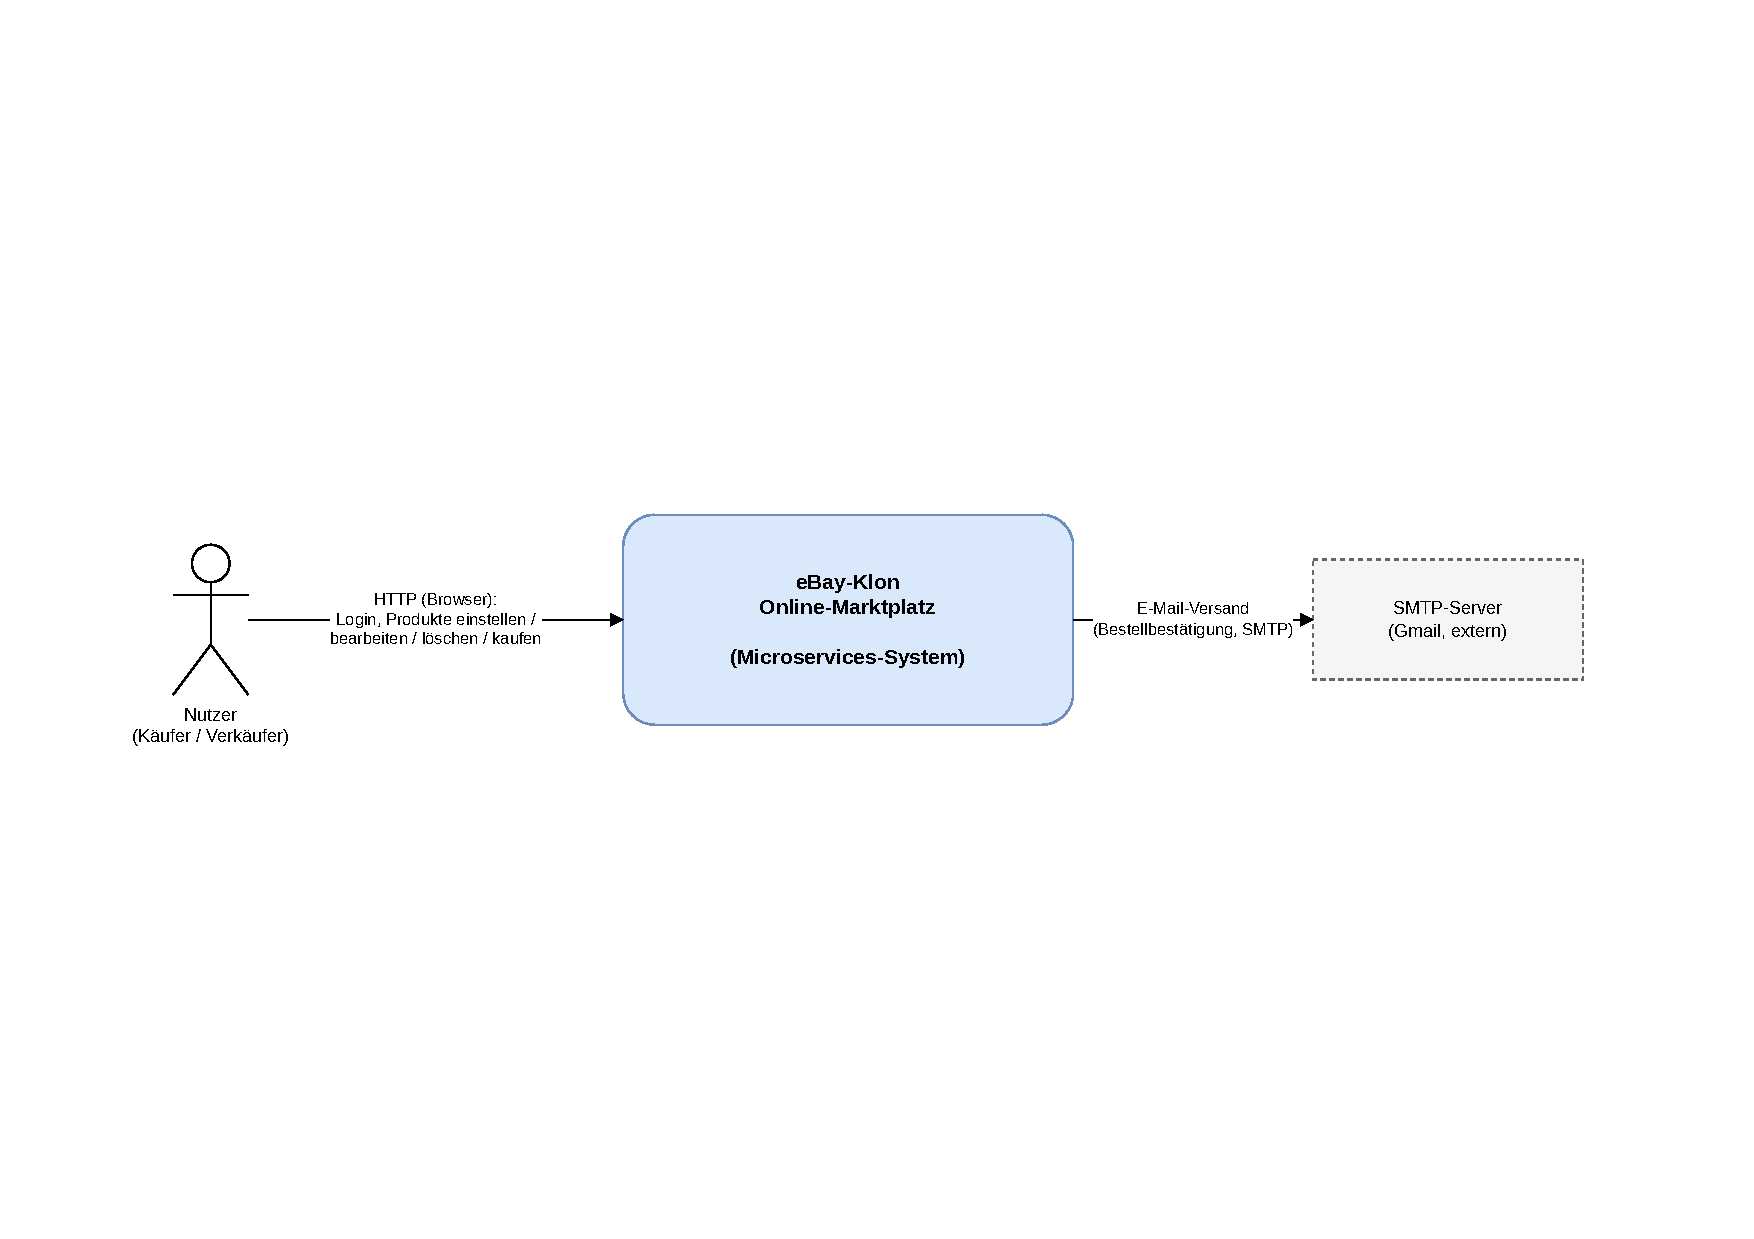
\includegraphics[width=\linewidth,trim=2cm 3cm 2cm 3cm,clip]{images/01-kontextdiagramm.pdf}
    \caption{Kontextdiagramm der E-Commerce-Plattform}
    \label{fig:kontextdiagramm}
\end{figure}